\paragraph{QuizziPedia::Front-End::Models::TrainingModeModel}
		
		\label{QuizziPedia::Front-End::Models::TrainingModeModel}
		
		\begin{figure}[ht]
			\centering
			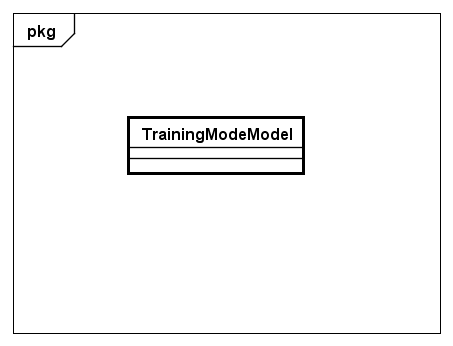
\includegraphics[scale=0.5,keepaspectratio]{UML/Classi/Front-End/QuizziPedia_Front-end_Models_TrainingModeModel.png}
			\caption{QuizziPedia::Front-End::Models::TrainingModeModel}
		\end{figure} \FloatBarrier
		
		\begin{itemize}
			\item \textbf{Descrizione}: rappresenta un allenamento. Contiene tutte le informazioni necessarie alla	presentazione del contenuto di un allenamento;
			\item \textbf{Utilizzo}: viene utilizzata per memorizzare i dati di un allenamento;
			\item \textbf{Relazioni con altre classi}: 
			\begin{itemize}
				\item \textbf{OUT} \texttt{TrainingController}: questa classe permette di gestire la modalità allenamento sottoponendo all'utente le giuste domande adatte al suo livello;
			\end{itemize}
			\item \textbf{Attributi}: 
			\begin{itemize}
				\item \texttt{- argument: String}\\
				Questo attributo rappresenta l'argomento dell'allenamento;
				\item \texttt{- keywords: Array<String>}\\
				Questo attributo rappresenta l'\texttt{array} contenente le parole chiave per l'allenamento;
				\item \texttt{- numberOfQuestions: Number}\\
				Questo attributo rappresenta il numero di domande che l'utente si è prefissato di rispondere per l'allenamento. Se \texttt{-1} allora non esiste un numero di domande impostate, perciò l'allenamento non terminerà fino alla chiusura manuale dell'attività;
				\item \texttt{- questions: Array<QuestionItemModel>}\\
				Questo attributo contiene l'\texttt{array} di \texttt{QuestionItemModel} che rappresenta le domande dell'allenamento fino a quel momento visualizzate, compresa quella visualizzata;
				\item \texttt{- rightAnswer: Number}\\
				Questo attributo rappresenta il numero di domande corrette date.
			\end{itemize}
			\item \textbf{Metodi}: 
			\begin{itemize}
				\item \texttt{+ setArgument(argument: String): void} \\
				Metodo \textit{setter\ped{G}} per il campo dati \texttt{argument}.\\
				\textbf{Parametri}:
				\begin{itemize}
					\item {argument: String}\\
					Questo parametro contiene l'argomento dell'allenamento.
				\end{itemize}
				
				\item \texttt{+ setNumberOfQuestions(numberOfQuestions: Number): void} \\
				Metodo \textit{setter\ped{G}} per il campo dati \texttt{numberOfQuestions}.\\
				\textbf{Parametri}:
				\begin{itemize}
					\item {author: ObjectId}\\
					Questo parametro rappresenta l'autore che ha creato la domanda.
				\end{itemize}
				
				\item \texttt{+ getArgument(): String} \\
				Metodo \textit{getter\ped{G}} che restituisce l'argomento dell'allenamento;
				
				\item \texttt{+ getNumeberOfQuestions(): Number} \\
				Metodo \textit{getter\ped{G}} che restituisce il campo dati \texttt{numeberOfQuestions};
				
				\item \texttt{+ addQuestion(question: QuestionItemModel): ObjectId} \\
				Metodo per aggiungere una domanda all'\texttt{array} di domande.\\
				\textbf{Parametri}:
				\begin{itemize}
					\item {question: QuestionItemModel}\\
					Questo parametro rappresenta la domanda da inserire.
				\end{itemize}
				
				\item \texttt{+ removeQuestion(idQuestion: ObjectId): void} \\
				Metodo per poter eliminare una domanda dall'allenamento.\\
				\textbf{Parametri}:
				\begin{itemize}
					\item {idQuestion: ObjectId}\\
					Questo parametro rappresenta l'id della domanda che si vuole rimuove dall'allenamento.
				\end{itemize}
				
				\item \texttt{+ addKeyword(keyword: String): void} \\
				Metodo per aggiungere una parola chiave all'array di parole chiavi.\\
				\textbf{Parametri}:
				\begin{itemize}
					\item {keyword: String}\\
					Questo parametro rappresenta la parola chiave da inserire.
				\end{itemize}
				
				\item \texttt{+ removeKeyword(keyword: String): void} \\
				Metodo per poter eliminare una parola chiave dall'array di parole chiavi.\\
				\textbf{Parametri}:
				\begin{itemize}
					\item {keyword: String}\\
					Questo parametro rappresenta la parola chiave da eliminare.
				\end{itemize}
				
				\item \texttt{+ getResult(): Object} \\
				Metodo \textit{getter\ped{G}} che restituisce risultato fino a quel momento dell'allenamento, ritornando un oggetto contenente il numero di domande giuste e totali.
				
			\end{itemize}
		\end{itemize}
			
		